\documentclass{standalone}
\usepackage{tikz}


\usepackage{xcolor}

\definecolor{purp}{RGB}{142,124,195}
% == Tikz
\newcommand{\drawcirc}{\node[draw,circle,minimum size=1.5cm]}
\newcommand{\drawbox}{\node[draw,rectangle,minimum size=1.5cm]}
\newcommand{\drawcircred}{\node[thick, red, draw,circle,minimum size=1.5cm]}
\newcommand{\drawcircpurp}{\node[thick, purp, draw,circle,minimum size=1.5cm]}
\newcommand{\drawcircblue}{\node[thick, blue, draw,circle,minimum size=1.5cm]}
\newcommand{\drawboxred}{\node[thick, red, draw,rectangle,minimum size=1.5cm]}
\newcommand{\drawboxpurp}{\node[thick, color=purp, draw,rectangle,minimum size=1.5cm]}
\newcommand{\drawdummy}{\node[minimum size=0,inner sep=0]}
\newcommand{\redarr}{\draw[thick, red, ->]}
\newcommand{\arr}{\draw[->]}
\newcommand{\midline}{\draw[-]}
\newcommand{\redmid}{\draw[thick, red, -]}
\newcommand{\bluearr}{\draw[thick, blue, ->]}
\newcommand{\bluemid}{\draw[thick, blue, -]}
\newcommand{\midlinered}{\redmid}
\newcommand{\midlineblue}{\bluemid}
\newcommand{\arrblue}{\bluearr}
\newcommand{\arrred}{\redarr}
\newcommand{\arrpurp}{\draw[thick, color=purp, ->]}
\newcommand{\midlinepurp}{\draw[thick, color=purp, -]}
\newcommand{\arrpurpultra}{\draw[ultra thick, color=purp, ->]}

% == Game
\newcommand{\zeroSink}{\mathsf{o}}
\newcommand{\target}{\mathsf{f}}
\newcommand{\val}{\mathsf{V}}

\begin{document}
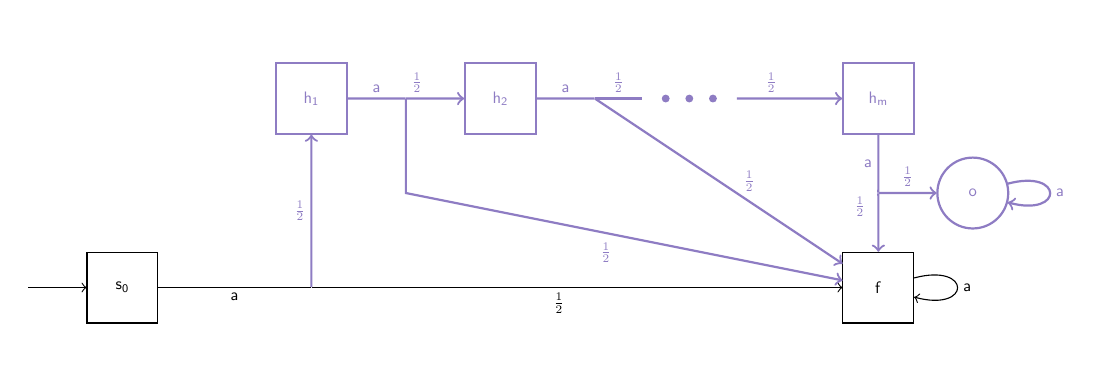
\begin{tikzpicture}[scale=0.6, every node/.style={transform shape}]
%little BCEC with loop
\drawdummy (init) at (-2,0) {};
\drawdummy (space1) at (0,5.5) {};
\drawdummy (space2) at (0,-1.5) {};
\drawbox (s0) at (0,0) {$\mathsf{s_0}$};
\drawbox (s1) at (16,0) {$\target$};
\drawdummy (s0Mid) at (4,0) {};

\drawboxpurp (m1) at (4,4) {$\mathsf{h_1}$};
\drawdummy (m1Mid) at (6,4) {};
\drawboxpurp (m2) at (8,4) {$\mathsf{h_2}$};
\drawdummy (m2Mid) at (10,4) {};
\drawdummy (helper1) at (11,4) {};
\drawdummy (helper2) at (13,4) {};
\drawboxpurp (m3) at (16,4) {$\mathsf{h_m}$};
\drawdummy (m3Mid) at (16,2) {};
\drawcircpurp (0) at (18,2)  {$\mathrm{\zeroSink}$};

\filldraw[color=purp] 
(11.5,4) circle (2pt)
(12,4) circle (2pt) 
(12.5,4) circle (2pt);

%\drawbox (1) at (4,4) {$\target$ };

\draw[->] (init) to (s0);
\draw[-] (s0) to node [below ,midway] {$\mathsf{a}$}(s0Mid);
\draw[->] (s0Mid) to node [text width =1.0cm, align=left, midway, below] {$\frac{1}{2}$} (s1);
\arrpurp (s0Mid) to node [midway, left] {$\frac{1}{2}$} (m1);

\midlinepurp (m1) to node [above,midway] {$\mathsf{a}$}(m1Mid);
\arrpurp (m1Mid) to (6,2) to node [text width =1.0cm, midway, below] {$\frac{1}{2}$} (s1);
\arrpurp (m1Mid) to node [text width =1.0cm, midway, above] {$\frac{1}{2}$} (m2);

\midlinepurp (m2) to node [above,midway] {$\mathsf{a}$}(m2Mid);
\arrpurp (m2Mid) to node [text width =-1.0cm, midway, right] {$\frac{1}{2}$} (s1);
\midlinepurp (m2Mid) to node [midway, above] {$\frac{1}{2}$} (helper1);
\arrpurp (helper2) to node [text width =1.0cm, midway, above] {$\frac{1}{2}$} (m3);

\midlinepurp (m3) to node [left,midway] {$\mathsf{a}$}(m3Mid);
\arrpurp (m3Mid) to node [text width =1.0cm, midway, above] {$\frac{1}{2}$} (s1);
\arrpurp (m3Mid) to node [midway, above] {$\frac{1}{2}$} (0);

\draw[->]  (s1) to [loop right] node [midway,right] {$\mathsf{a}$} (s1);
\arrpurp  (0) to [loop right] node [midway,right] {$\mathsf{a}$} (0);
\end{tikzpicture}
\end{document}
